\section{Preparing for implementation}
\label{sec:primarythoughts}

After looking at challenges and possible solutions to them, a few keywords are essential:

\begin{description}
  \item[Remote] -- Outsorce long-lasting actions to an external service.
  \item[Cache] -- Speed up builds by making use of already finished work.
  \item[Versioning] -- Keep track on development and possibly revert, if necessary.
  \item[Branches] -- Let different parts of development evolve to their own speed.
\end{description}

While it may appear, that the above list is too fixated on version control systems, it should be clear now, that especially Git qualifies core companion to any website project, especially when the project itself is maintained by multiple developers, designers and/or authors. Being aware of GitHub as social code management tool and moreover the benefits of its API, the foundation stone should be laid (see ch. \ref{sec:solutions-distributeddevelopment} on p. \pageref{sec:solutions-distributeddevelopment}).

%% Graphic of basic api flow
\begin{figure} % h-ere, t-op, b-ottom, p-age
    \centering
    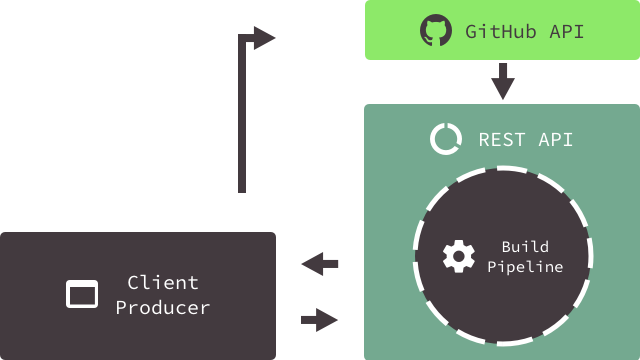
\includegraphics[width=0.75\textwidth]{api_flow.png}
    \caption{An abstract flow visualization of the planned request cycle. The client (developer, content creator) manages his/her code on GitHub. Based on the respective configuration, a build cycle may be triggered either using a GitHub webhook, or by manually sending a POST request to a certain endpoint.    That request then gets caught by the REST API, which creates an instance of the build pipeline. The pipeline requests data of the project from GitHub and sets up the project configuration. After a successful build, the REST API provides a downloadable archive of the newly built webroot.}
    \label{fig:api-flow}
\end{figure}
%

Since the tool should also be remotely accessible, it makes sense to also design it as RESTful API, for handling programmatical access as well as access from possible frontend apps lying on top. Furthermore, its main work cycle might get detached for neither distracting users due to ordering them to wait until it finished, nor blocking access in between (see Fig. \ref{fig:api-flow}).

However, the most important part behind these thoughts is the choice of the ideal static site generator.


\subsection{Choosing a static site generator}
\label{sec:primarythoughts-generator}

Due to the fact, that the choice of the best possible static site generator is the linchpin for a project like this, the evaluation needs to cover its usability, pluggability, customizability and overall maintenance, as well as the level of its general support. First and foremost, the installation process should be as easy as possible and not rely on too many third-party dependencies, which are probably not needed afterwards. Through this, it may be guaranteed, that also users, who are foreign to development, are likely to set up an instance on their local machines, although not critically required. This creates awareness for the project structure and therefore may lead to less support requests in the future.

The programming language of the chosen static site generator does have to be considered well, as it has to fit seamlessly into a planned REST API, in the best case without any further adapter in between. This should make it also easy to hook additional code into the configuration step, if needed. Ideally, it emits events as well, so any host process knows when a detached process is finished.

All in all, the best possible solution seems to be \emph{Metalsmith} (see ch. \ref{sec:metalsmith} on p. \pageref{sec:metalsmith}), as it not only offers a pluggable module ecosystem, but also access to a JavaScript API, among others. Together with some custom tweaks (e.g. dynamic module loading), an independent build setup for each project may be injected using only a specific configuration file.


\subsection{Constructing a REST API}
\label{sec:primarythoughts-restapi}

JavaScript proved its universality due to its usage both on client- and server-side, thus, a major advantage is its common knowledge among developers combined with a low barrier to entry for people, which are already found in frontend-development.

Node.js is a server-side implementation for JavaScript, backed by Google's V8 engine, which directly translates the scripting language into machine code \cite[4]{cantelon2017node}. This perfetly supports developers in reducing their tradeoff for possibly having to handle multiple ecosystems at once. A seamless integration of Metalsmith into the API service may therefore happen without much hassle.

The easy installation is supported by several third-party apps like Node Version Manager (\emph{NVM})\footnote{\url{https://github.com/creationix/nvm} -- NVM's repository on GitHub.} and mostly will not need any admin rights, which makes it ideal to use on hosting environments without root access (unlike PHP or Ruby for example). Although not equally well supported among the most popular operating systems, at least MacOS and Linux provide a stable enough environment for NVM.

Looking for a framework for setting up an API, \emph{Express}\footnote{\url{http://expressjs.com/} -- Website of Express.} seems to be the perfect fit, as it consists only of a very basic setup -- similar to Metalsmith -- but may be easily enhanced using different node modules, thus providing a uniquely shaped web application in contrast to conventional, monolithic frameworks like \emph{Django} or \emph{Ruby on Rails} \cite[176]{cantelon2017node}.

% Express sample basic configuration
\lstinputlisting[caption={An example for a basic express.js setup, roughly taken from \url{http://expressjs.com/en/starter/hello-world.html}.\\
In this case, a web application listens for a \emph{GET} request on its root path ``/'' and responds with a ``Hello World!'' message.}, label={list:express-setup}, language=JavaScript]{chapters/04-theoretical-approach/_support/express.js}

As a result, the main purpose of such an express application would be acting as a web-based infrastructure for the underlying build pipeline. Based on different REST endpoints, as well as their request parameters, executing a uniquely configured Metalsmith process on a project directory within the API's file tree should be possible without any further external interaction requirement. The project directory would be provided using an appropriate GitHub repository, requiring only a basic, as little opinionated configuration as possible, together with a public access possibility to the repo.

Additionally, to benefit most from any remote outsourcing, a current production-ready version of the project may be held available at a special endpoint for downloading at any time. In this case, further processing is enabled without waiting for completion of any build cycle beforehand, unless the source code received any updates through development.


\subsection{Selective rendering}
\label{sec:primarythoughts-rendering}

While the theoretical foundations for a project covering the use case of static site generation are now defined, a constantly growing amount of necessary build time still remains as one of the core problems. Caching across remote machines is likely to be impossible, especially if local computers also have to be added to the caching network and not every node is working on the same project revision at the same time. Moreover, an additional distribution mechanism would also have to be implemented, acting primarily as supply tool for providing already rendered revisions of different steps in development.

If cutting down on expectations and concentrating on basic improvements of speeding up a build cycle, a solution without exchanging complete file trees might be possible. To make sure all required data is accessible, the respective GitHub API credentials are mandatory. The main reason behind that is the gapless availability of every commit and its underlying file tree via HTTP -- therefore a separate \texttt{git checkout} on server level is not needed, GitHub provides the according file tree as immediately obtainable tarball or zip archive.

Together with the development history between two individual commits resulting in a diff and a downloadable file tree representing a certain step in the current progress, a build log has to keep track of the ongoing rendering actions and their results. The idea behind that is the possibility of remembering any render action in the past and incrementally building up on the latest positive result by only selecting the modified files for use in the build pipeline and leave out any other. Relying on an already available bugless result of a previous build cycle, any successful outcome of an upcoming action based on a later commit may be easily merged (see ch. \ref{sec:solutions-caching} on p. \pageref{sec:solutions-caching}).
